\documentclass[10pt]{article} % dà errore perchè non trova citazioni, ignorabile perchè compila comunque
\usepackage[utf8]{inputenc}
\usepackage{listings}
\usepackage{xcolor}
\usepackage{subcaption}
\usepackage{longtable}
\usepackage{booktabs}
\usepackage{enumitem}
\usepackage{hyperref}

\hypersetup{
	colorlinks,
	citecolor=black,
	filecolor=black,
	linkcolor=black,
	urlcolor=black
}

\definecolor{codegreen}{rgb}{0,0.6,0}
\definecolor{codegray}{rgb}{0.5,0.5,0.5}
\definecolor{codepurple}{rgb}{0.58,0,0.82}
\definecolor{backcolour}{rgb}{0.95,0.95,0.92}
\usepackage{color}   %May be necessary if you want to color links
\usepackage{hyperref}
\usepackage{graphicx}
\usepackage{adjustbox}
\graphicspath{ {./images/} }
\hypersetup{
    colorlinks=true, %set true if you want colored links
    linktoc=all,     %set to all if you want both sections and subsections linked
    linkcolor=black,  %choose some color if you want links to stand out
    urlcolor=blue,
}
\lstdefinestyle{mystyle}{
    backgroundcolor=\color{backcolour},   
    commentstyle=\color{codegreen},
    keywordstyle=\color{magenta},
    numberstyle=\tiny\color{codegray},
    stringstyle=\color{codepurple},
    basicstyle=\ttfamily\footnotesize,
    breakatwhitespace=false,         
    breaklines=true,                 
    captionpos=b,                    
    keepspaces=true,                 
    numbers=left,                    
    numbersep=5pt,                  
    showspaces=false,                
    showstringspaces=false,
    showtabs=false,                  
    tabsize=2
}

\lstset{style=mystyle}

\bibliographystyle{plain}

\title{DD}
\author{Mauro Famà, Giacomo Lombardo}
%\date{October 2021}

\begin{document}
\thispagestyle{empty}
\begin{titlepage}
    \newcommand{\HRule}{\rule{\linewidth}{0.5mm}}
    \center
    
\includegraphics[width=8cm]{polimi.png}\\[1cm]

    \textsc{\Large Software Engineering II}\\[0.5cm]
    \textsc{\large A.Y. 2021/22}\\[0.5cm]

    \HRule \\[0.4cm]
        { \Huge \bfseries DREAM}\\[0.2cm]
        { \large Data-dRiven prEdictive fArMing}\\[0.4cm]
        { \LARGE Design Document}
    \HRule \\[1.5cm]

    \begin{minipage}{0.4\textwidth}
        \begin{flushleft} \large
        \emph{Authors:}\\
        Mauro \textsc{Famà}\\
        Giacomo \textsc{Lombardo}\\
        \end{flushleft}
    \end{minipage}\\[2cm]

    {\large January 9, 2022}\\[2cm]
    
    \vfill
\end{titlepage}
\newpage
\tableofcontents %this command creates an index
\newpage
\section{Introduction}
\subsection{Purpose}
The purpose of this document is to comprehensively describe the design of the DREAM platform. %(reference to rasd or assignment)
It will be described the architecture of the system and its characteristics, 
moreover will be analyzed its components explaining their functionalities.\\
This document was written following the RASD of the same project, 
in fact the assumptions and design choices are based on the assumptions already explained, 
however maintaining independence between the documents. This document focuses on the explanation 
about the Software-To-Be, its modules, its interfaces and its implementation.
\subsection{Scope}
The main objective of the platform is to create a support tool and communication channel for farmers in Telangana, 
leveraging the IT infrastructure of government resources. The platform also aims to be a 
supervisory and control system for the authorities of the Ministry of Agriculture in Telangana, 
providing accurate and bulk data of farmers' performance, reducing the overhead due to manual retrieval of this information.\\
The system will have two separate and exclusive interfaces, one dedicated to PMs in Telangana 
and one dedicated to farmers in the region. Farmers will be provided with a browser 
executable web application, it will provide a dashboard to monitor the sensors embedded 
in their fields, weather forecasts for the local area and summarize the resources 
obtained and consumed by the plantations. In addition to the monitoring functionality, 
from the farmer's dashboard it will be possible to compile reports to be sent to the PM 
responsible for the area, combining data entered manually by the farmer, data created by 
IoT devices and data retrieved from the internet.\\
The web application also provides access to the forum dedicated to the Telangana farming community, 
connecting all participants in the DREAM program through its threads.
Farmers will also be able to submit their help requests into the system, which will be automatically forwarded 
to the PM responsible for the area, who in turn will have a dedicated dashboard exclusively for the administrative side.
From his application, the PM will be able to forward responses to help requests, monitor the performance of 
farmers in his area, all while viewing data from sensors and weather forecasts.
From his dashboard, the PM will have the tools to perform end-of-quarter performance evaluations, 
including direct communication channels to affected farmers.\\
There is no platform that currently provides these functions, in fact this document refers to the design of a system 
created from scratch, without any integration of existing systems, but exploiting the IT infrastructure 
already physically installed in the Telangana region.

\subsection{Definitions, Acronyms, Abbreviations}
\subsection{Revision History}
\subsection{Reference Documents}
\subsection{Document Structure}
\section{Architectural Design}
\subsection{Overview}
\begin{figure}[h]
    \centering
    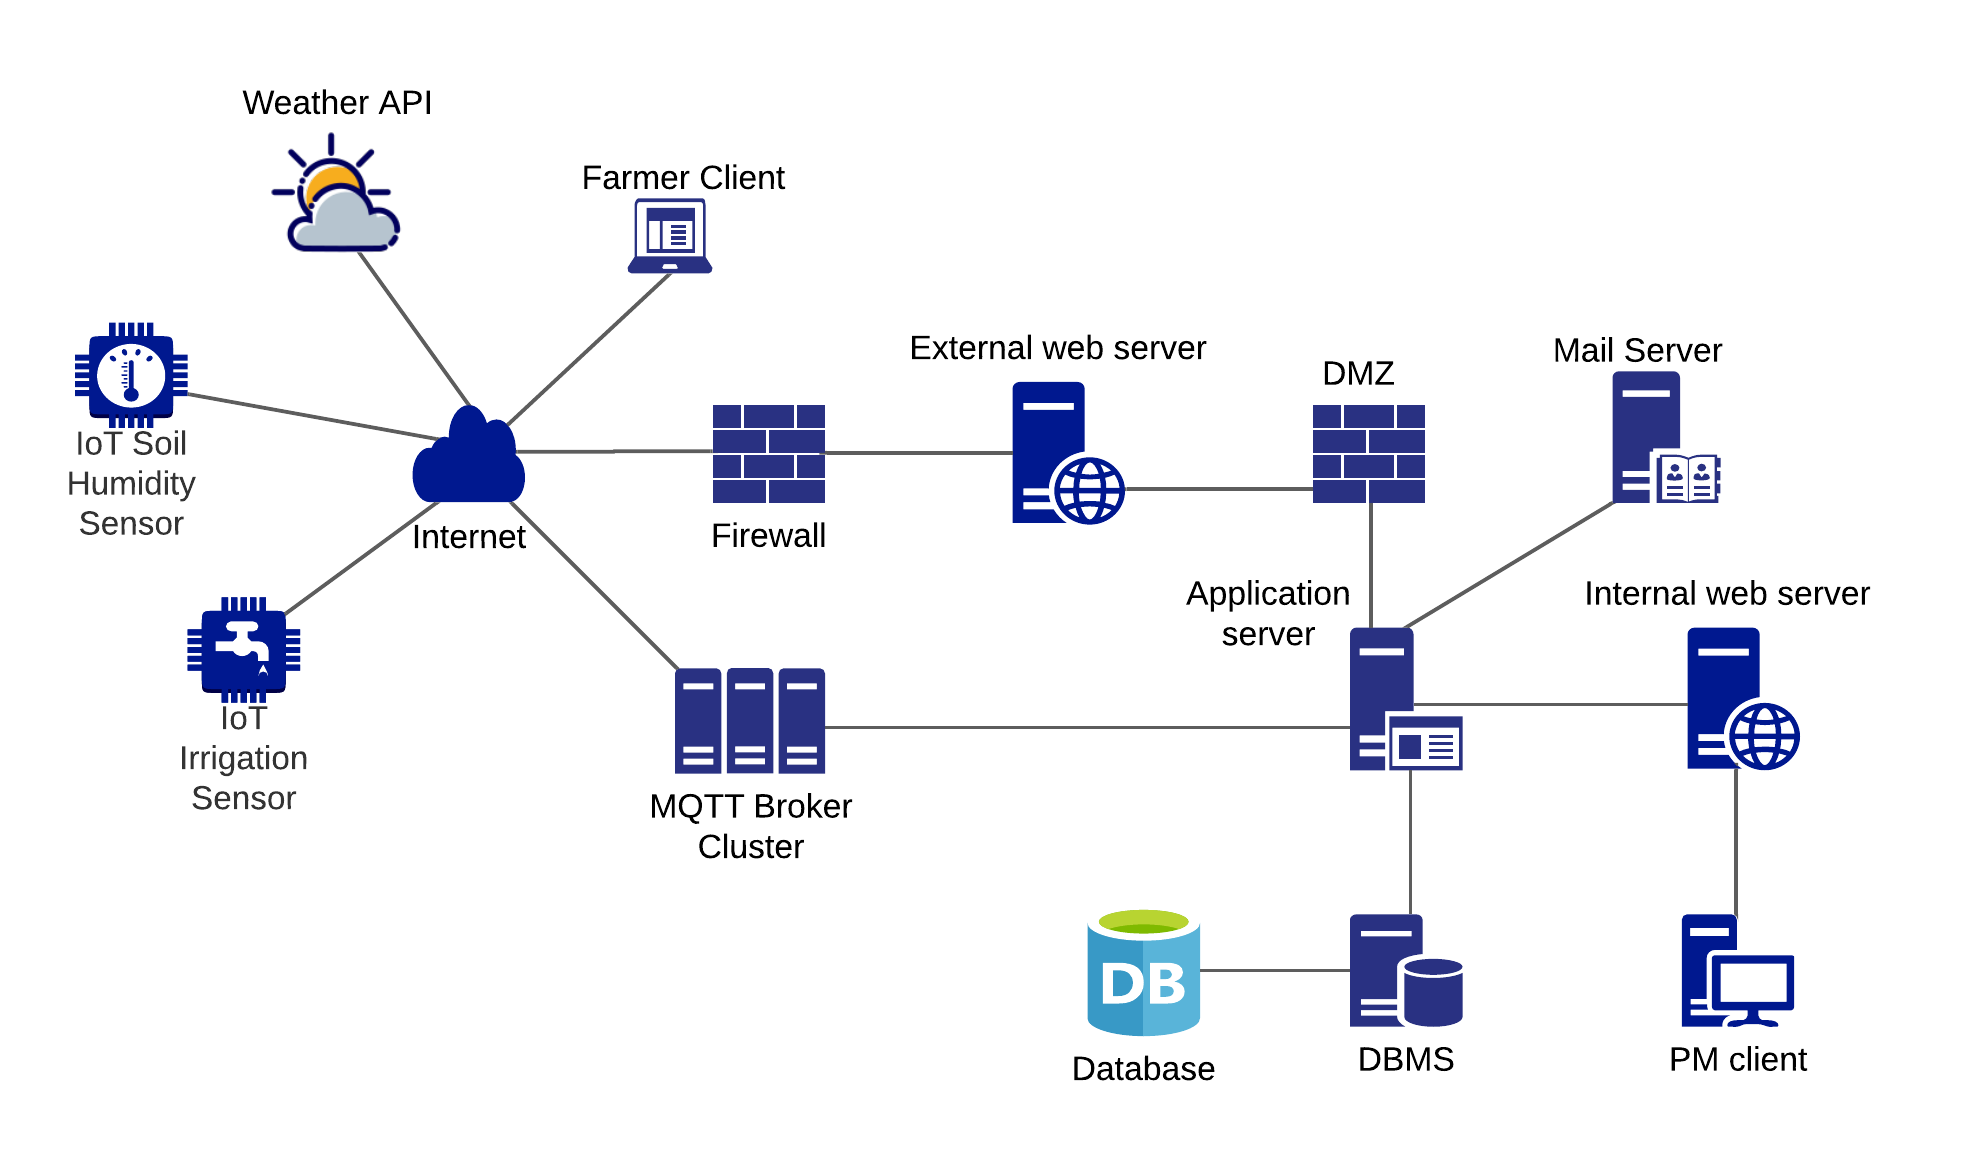
\includegraphics[scale=0.7]{images/overview_architecture.png}
    \caption{System architecture}
    \label{fig:overview}
\end{figure}
The system will be developed from scratch and it will entirely replace the legacy system.
The DREAM application is designed with as a three-tier application with web servers, application server, and a database functioning as the three tiers of the application.
The application can be accessed via a webapp provided both to internal and external users. The internal users of the application are the policy maker, that will log into and use the platform
from their workstation, connected to an internal web server. The external users are the farmer, connected to the webapp from their personal computer. This separation between internal and external 
users is meant first and foremost for security requirements, in order not to expose sensitive data to potential risks.\\
Other significant components in the DREAM ecosystem are the IoT sensors, crucial to automatically retrieve and collect data from local farmers and to better evaluate their performances.
IoT sensors are connected via MQTT protocol to a MQTT Broker Cluster which periodically retrieves the data collected by sensors.\\
All the weather informations are taken from the weather forecasting system of Telangana through its APIs.\\
Finally, the application server communicate with a database through a Database Management System.\\
A more detailed description of the components will be given in the following sections.
\subsection{Component view}
\begin{figure}[h]
    \centering
    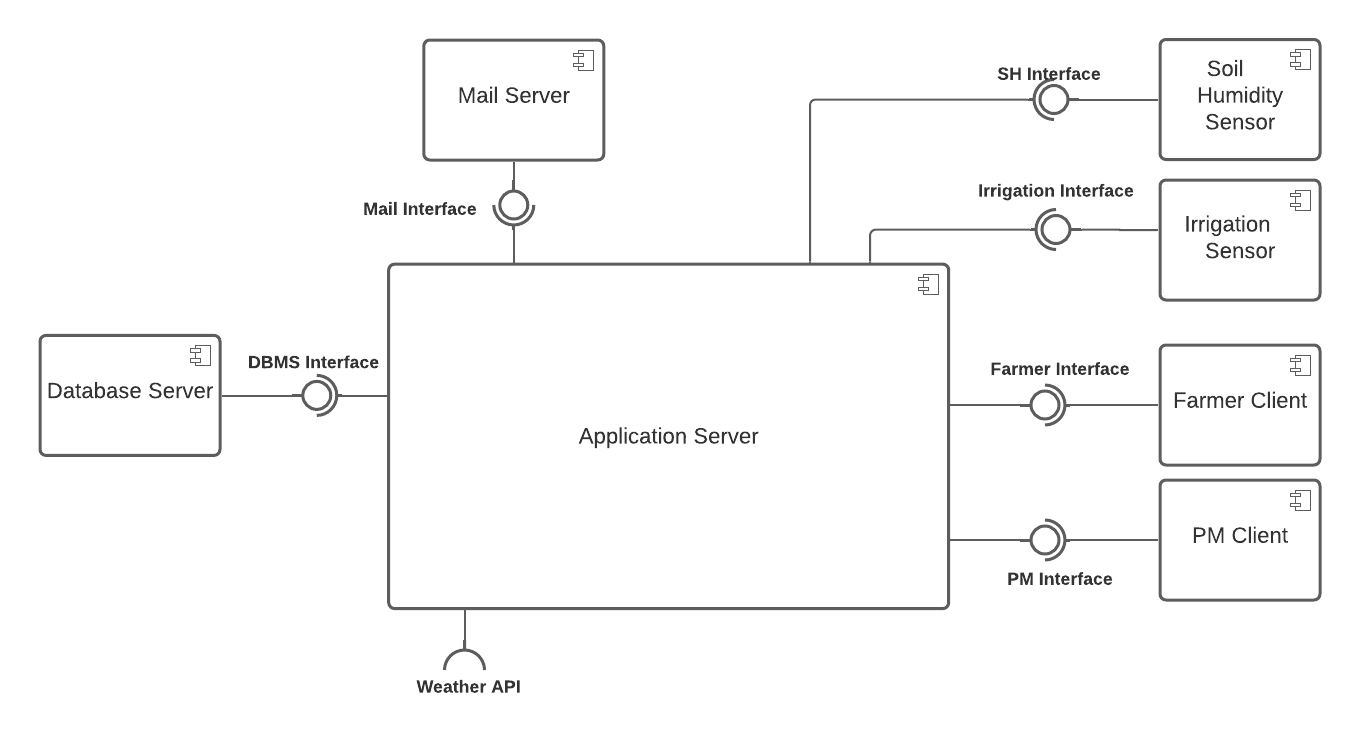
\includegraphics[scale=0.43]{images/hl_component.png}
    \caption{High Level Component Diagram}
    \label{fig:hl_component}
\end{figure}
\begin{itemize}
    \item \textbf{Database server}\\This component is responsible for data management, 
    it provides the interface of the Database Management System to the Application Server, in order to 
    deal with the data management, storing and modification process.
    \item \textbf{Mail server}\\This component allows the Application Server to create and manage email accounts, 
    send and receive email using standard email protocols. The SMTP protocol is used to send messages and handle outgoing mail requests, 
    The IMAP protocol is used to receive messages and to process incoming mail.
    \item \textbf{Application server}\\It is the main component of the system, all the business logic 
    resides in it. This component offers both functionality dedicated to farmers and PMs, 
    interfacing directly with clients. It receives the data entered by the users and sent 
    by the weather forecast system, cross-referencing them and providing for processing, 
    back forwarding and transferring them to the data management system. Its components are 
    described in detail in the following sections.
    \item \textbf{Farmer client}\\It is the component thanks to which the farmers can interface 
    with the Application Server. It represents the web application dedicated to farmers that allows 
    them to access the services of DREAM. This component also receives data from the IoT sensors that 
    monitor the farmer's possessions, making them available to be retrieved from to the Application Server.
    \item \textbf{PM client}\\This is the component thanks to which the Policy Makers can interface 
    with the Application Server. It represents the web application dedicated to them that allows 
    them to take advantage of the services offered by DREAM to monitor and manage agriculture in 
    Telangana. All the functions are accessible thanks to the PM Interface exposed by the Application Server.
    \item \textbf{Soil Humidity and Irrigation sensors}\\
    Sensors for measuring soil humidity and irrigation are 
    internet-connected components responsible for creating and sending data about farmers metrics to the Application Server. 
    They both expose their own interface, through which the Application Server can retrieve the data of interest.
\end{itemize}
\subsubsection{Application Server}
The application server contains the business logic of the application. The following diagram describe its internal structure:
\begin{figure}[h]
    \centering 
    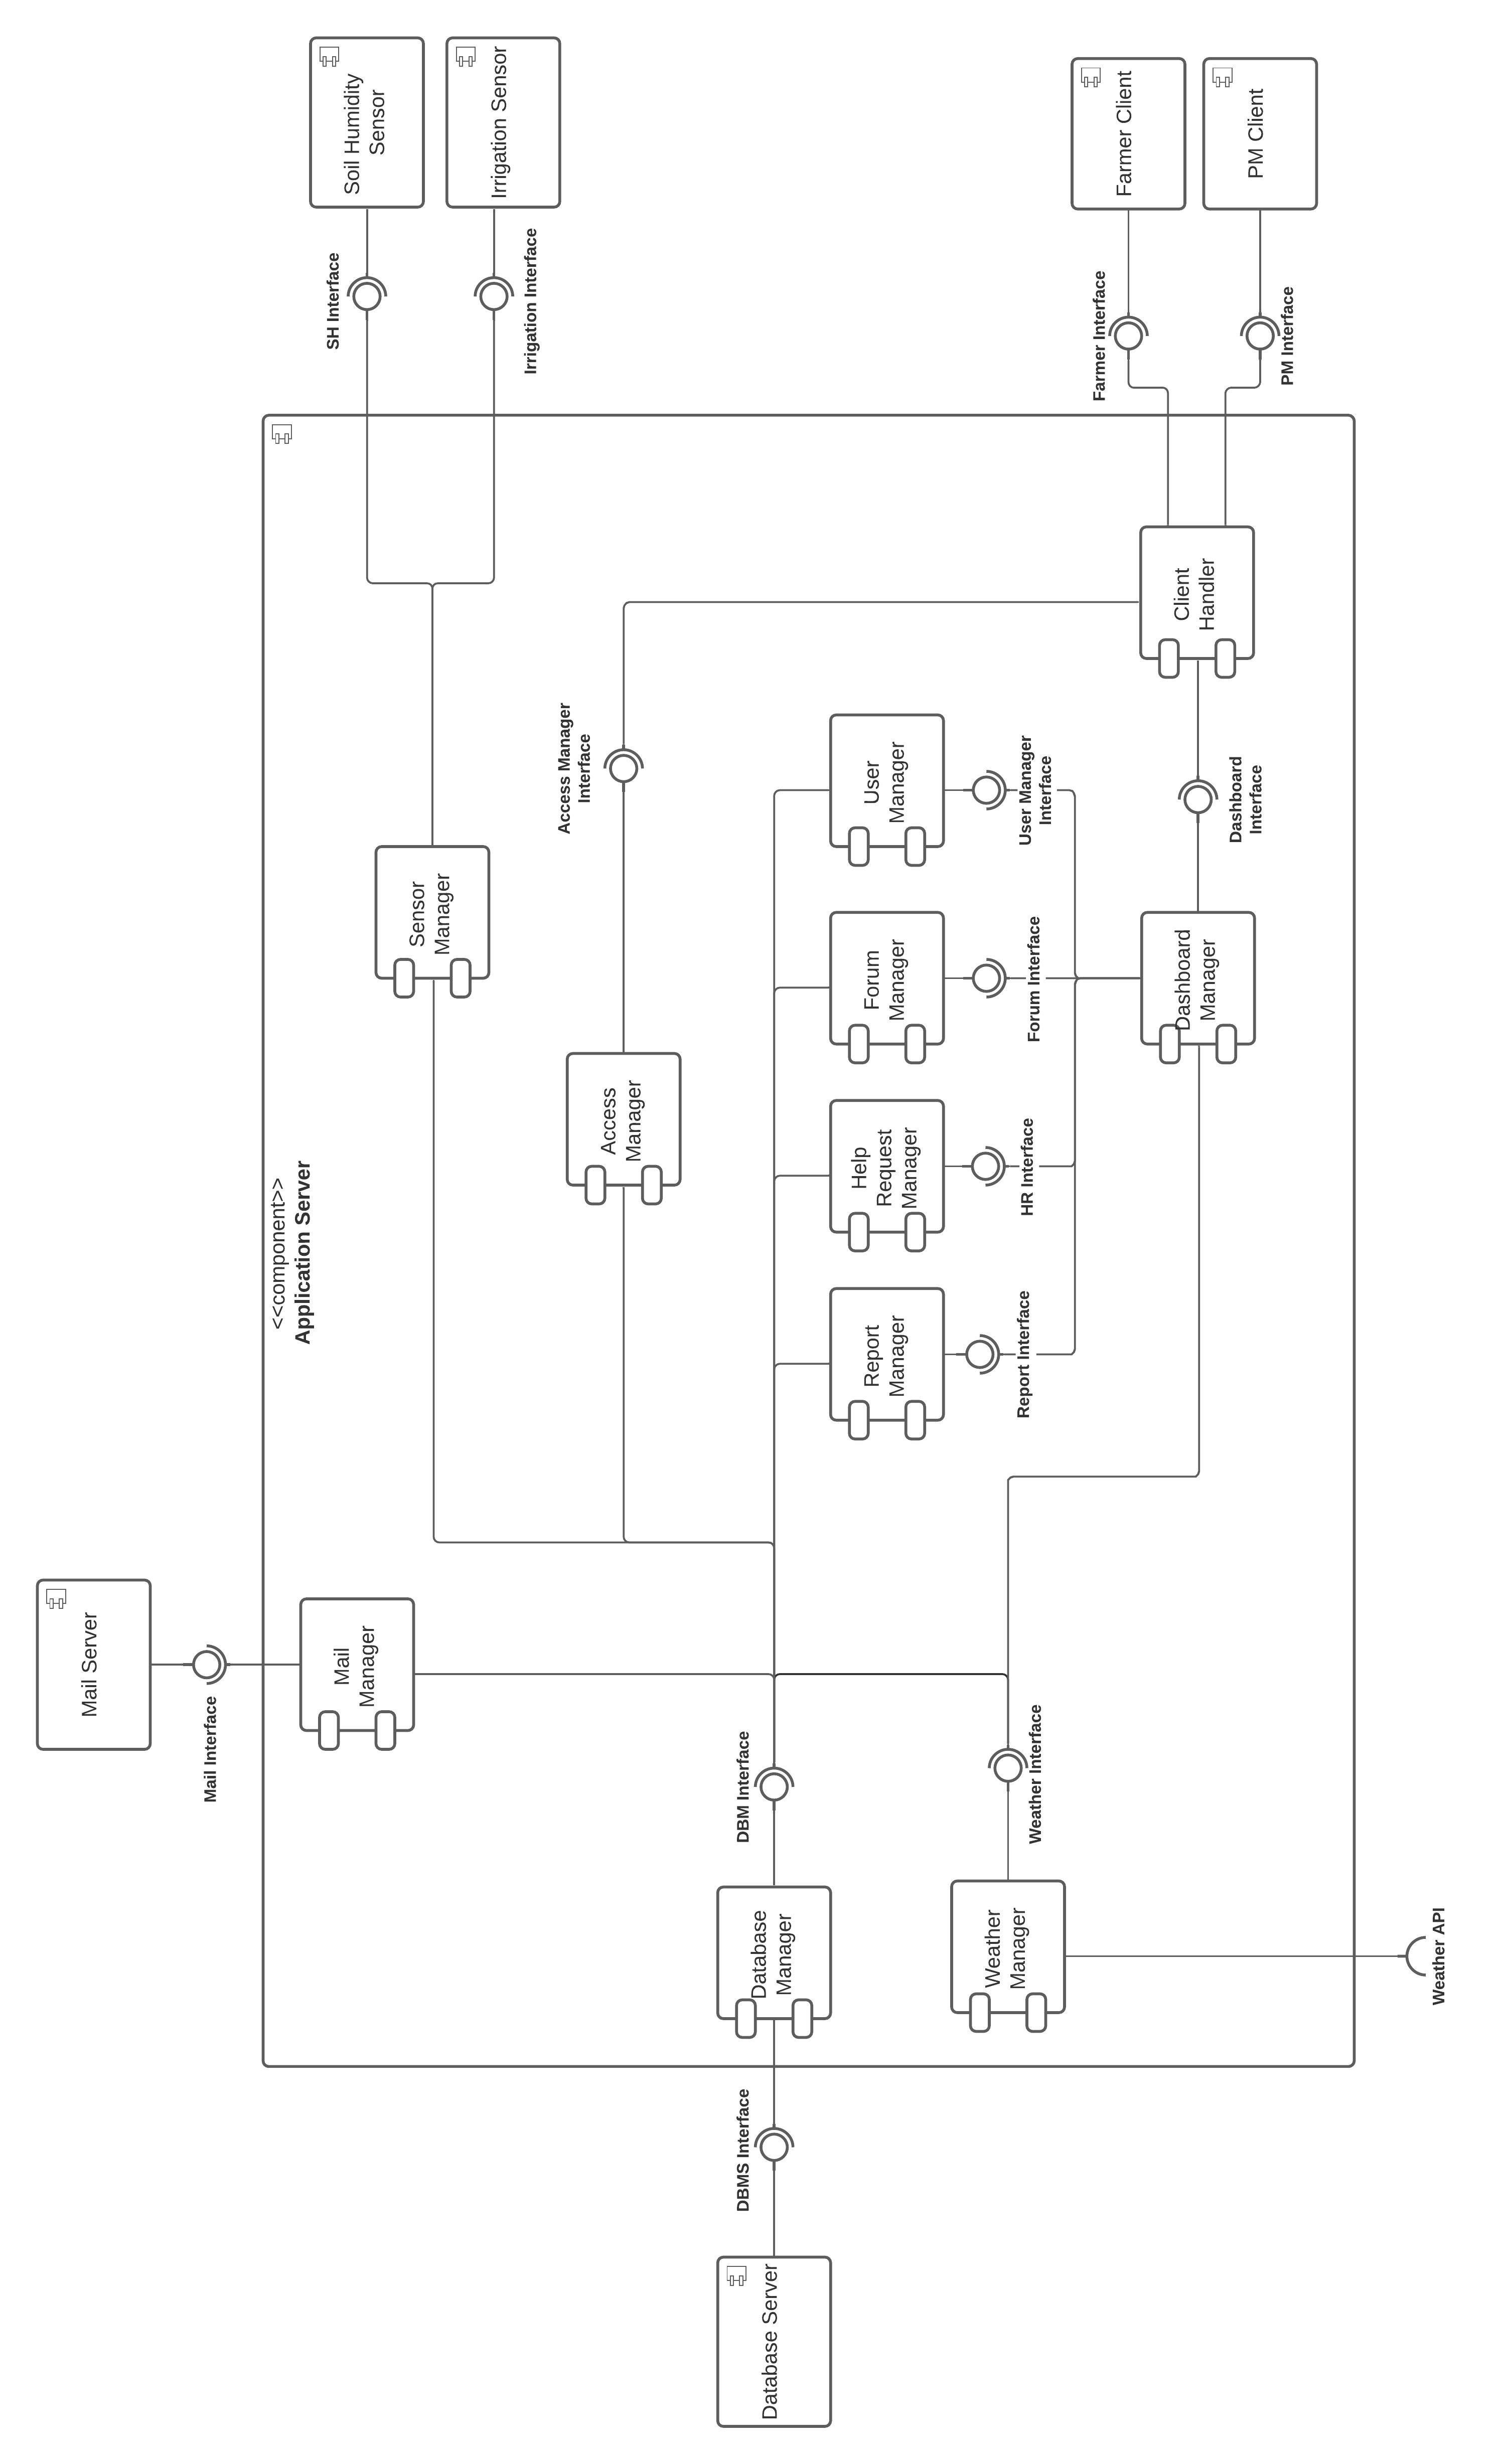
\includegraphics[scale=0.38]{images/app_server_component.png}
    \caption{Application Server Component Diagram}
    \label{fig:app_component}
\end{figure}
The components of the application server are:
\begin{itemize}
    \item \textbf{Database Manager}: deals with management of the data model and data operations, working as a bridge between the physical database 
    and the other components of the server.
    \item \textbf{Mail Manager}: interfaces between the server components and the mail server in order to provide mailing services.
    \item \textbf{Weather Manager}: interfaces between the external weather forecasting API and the other server components.
    \item \textbf{Access Manager}: handles the authentication procedure of the application's users. It is also responsible for the generation of access credentials.
    \item \textbf{Sensor Manager}: handles the communications between the application and the sensors installed in the Telangana territory. Manages the retrieving of 
        collected data from the sensors and its processing and storing procedure.
    \item \textbf{Report Manager}: handles the creation and the visualization of reports.
    \item \textbf{Help Request Manager}: handles the creation, the handling and the visualization of help requests.
    \item \textbf{Forum Manager}: handles forum operations such as creation of threads, answering, visualization and moderation.
    \item \textbf{User Manager}: manages the retrieving of user information from the database.
    \item \textbf{Dashboard Manager}: manages the process of generation of web pages, retrieving the necessary data from the other interfaces, and the handling of user requests. 
        This component will be further analyzed in the following part of the document.
    \item \textbf{Client Handler}: handles clients' connection, interfacing between the application server and the clients.
\end{itemize}
\subsubsection{Client Handler}
\begin{figure}[h]
    \centering 
    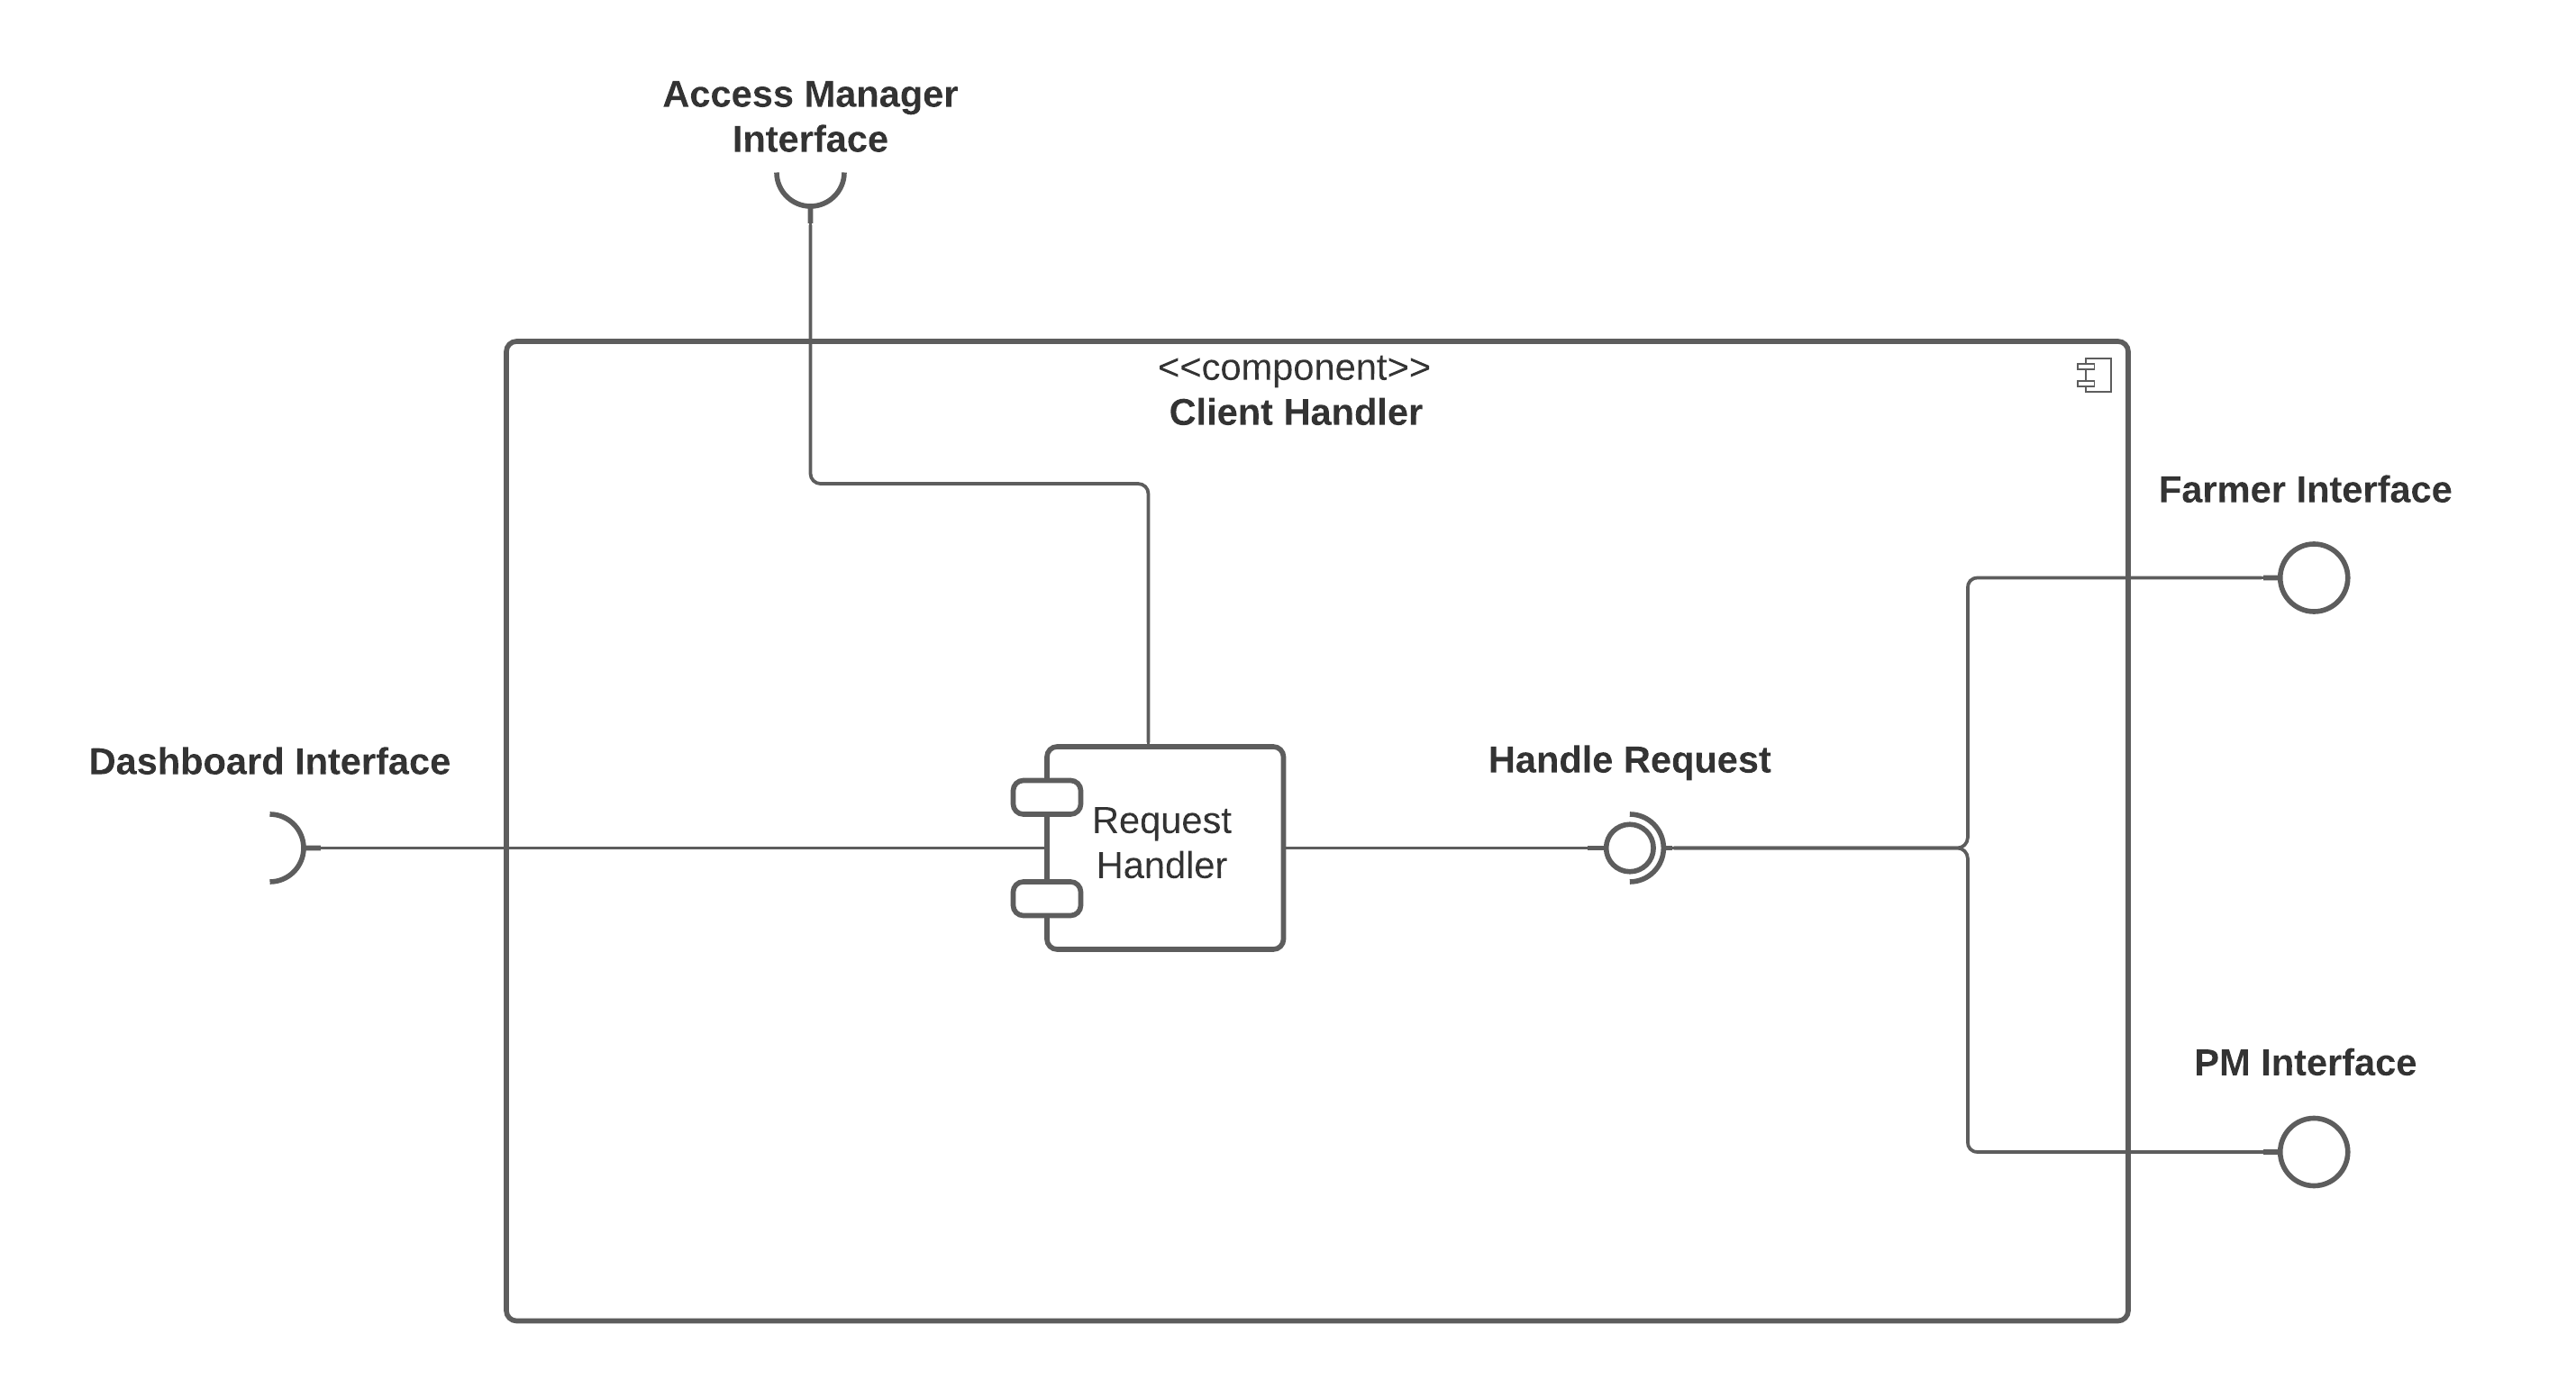
\includegraphics[scale=0.5]{images/clientHandler.png}
    \caption{Client Handler Component Diagram}
    \label{fig:client_handler}
\end{figure}
\subsubsection{Dashboard Manager}
\begin{figure}[h]
    \centering 
    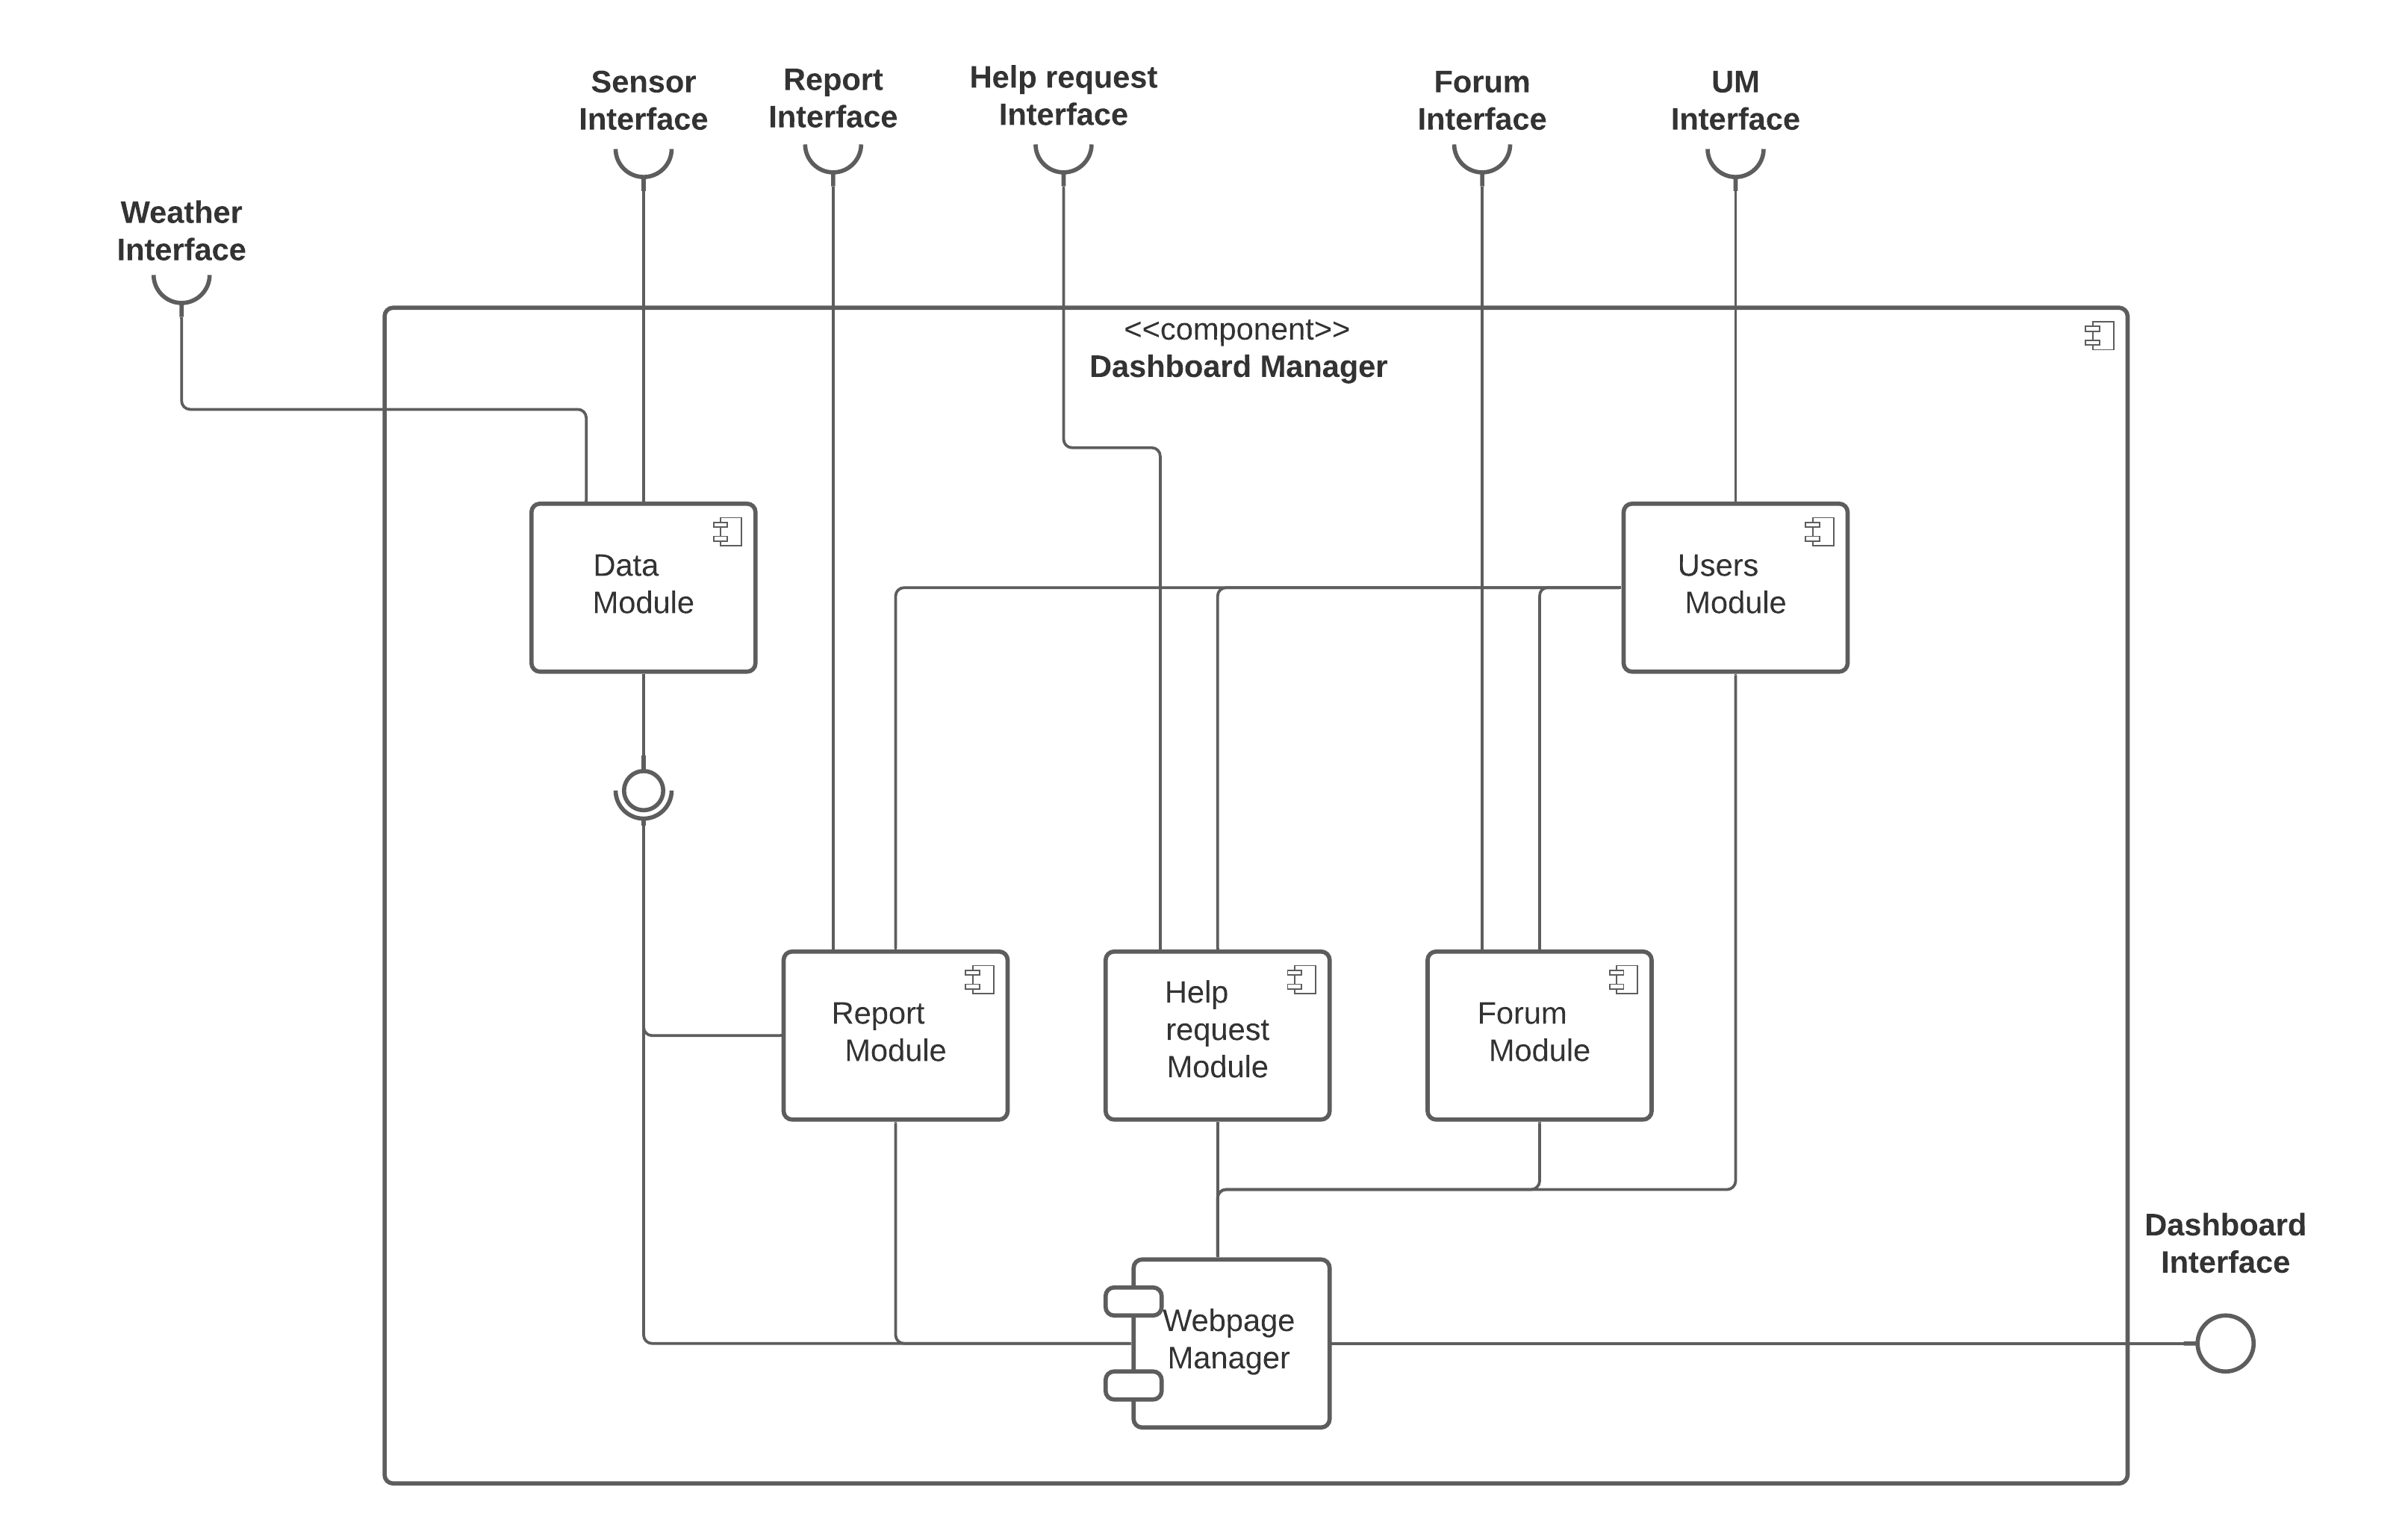
\includegraphics[scale=0.4]{images/dashboardManager.png}
    \caption{Dashboard Manager Component Diagram}
    \label{fig:dashboard_manager}
\end{figure}
\subsection{Deployment view}
\begin{figure}[h]
    \centering
    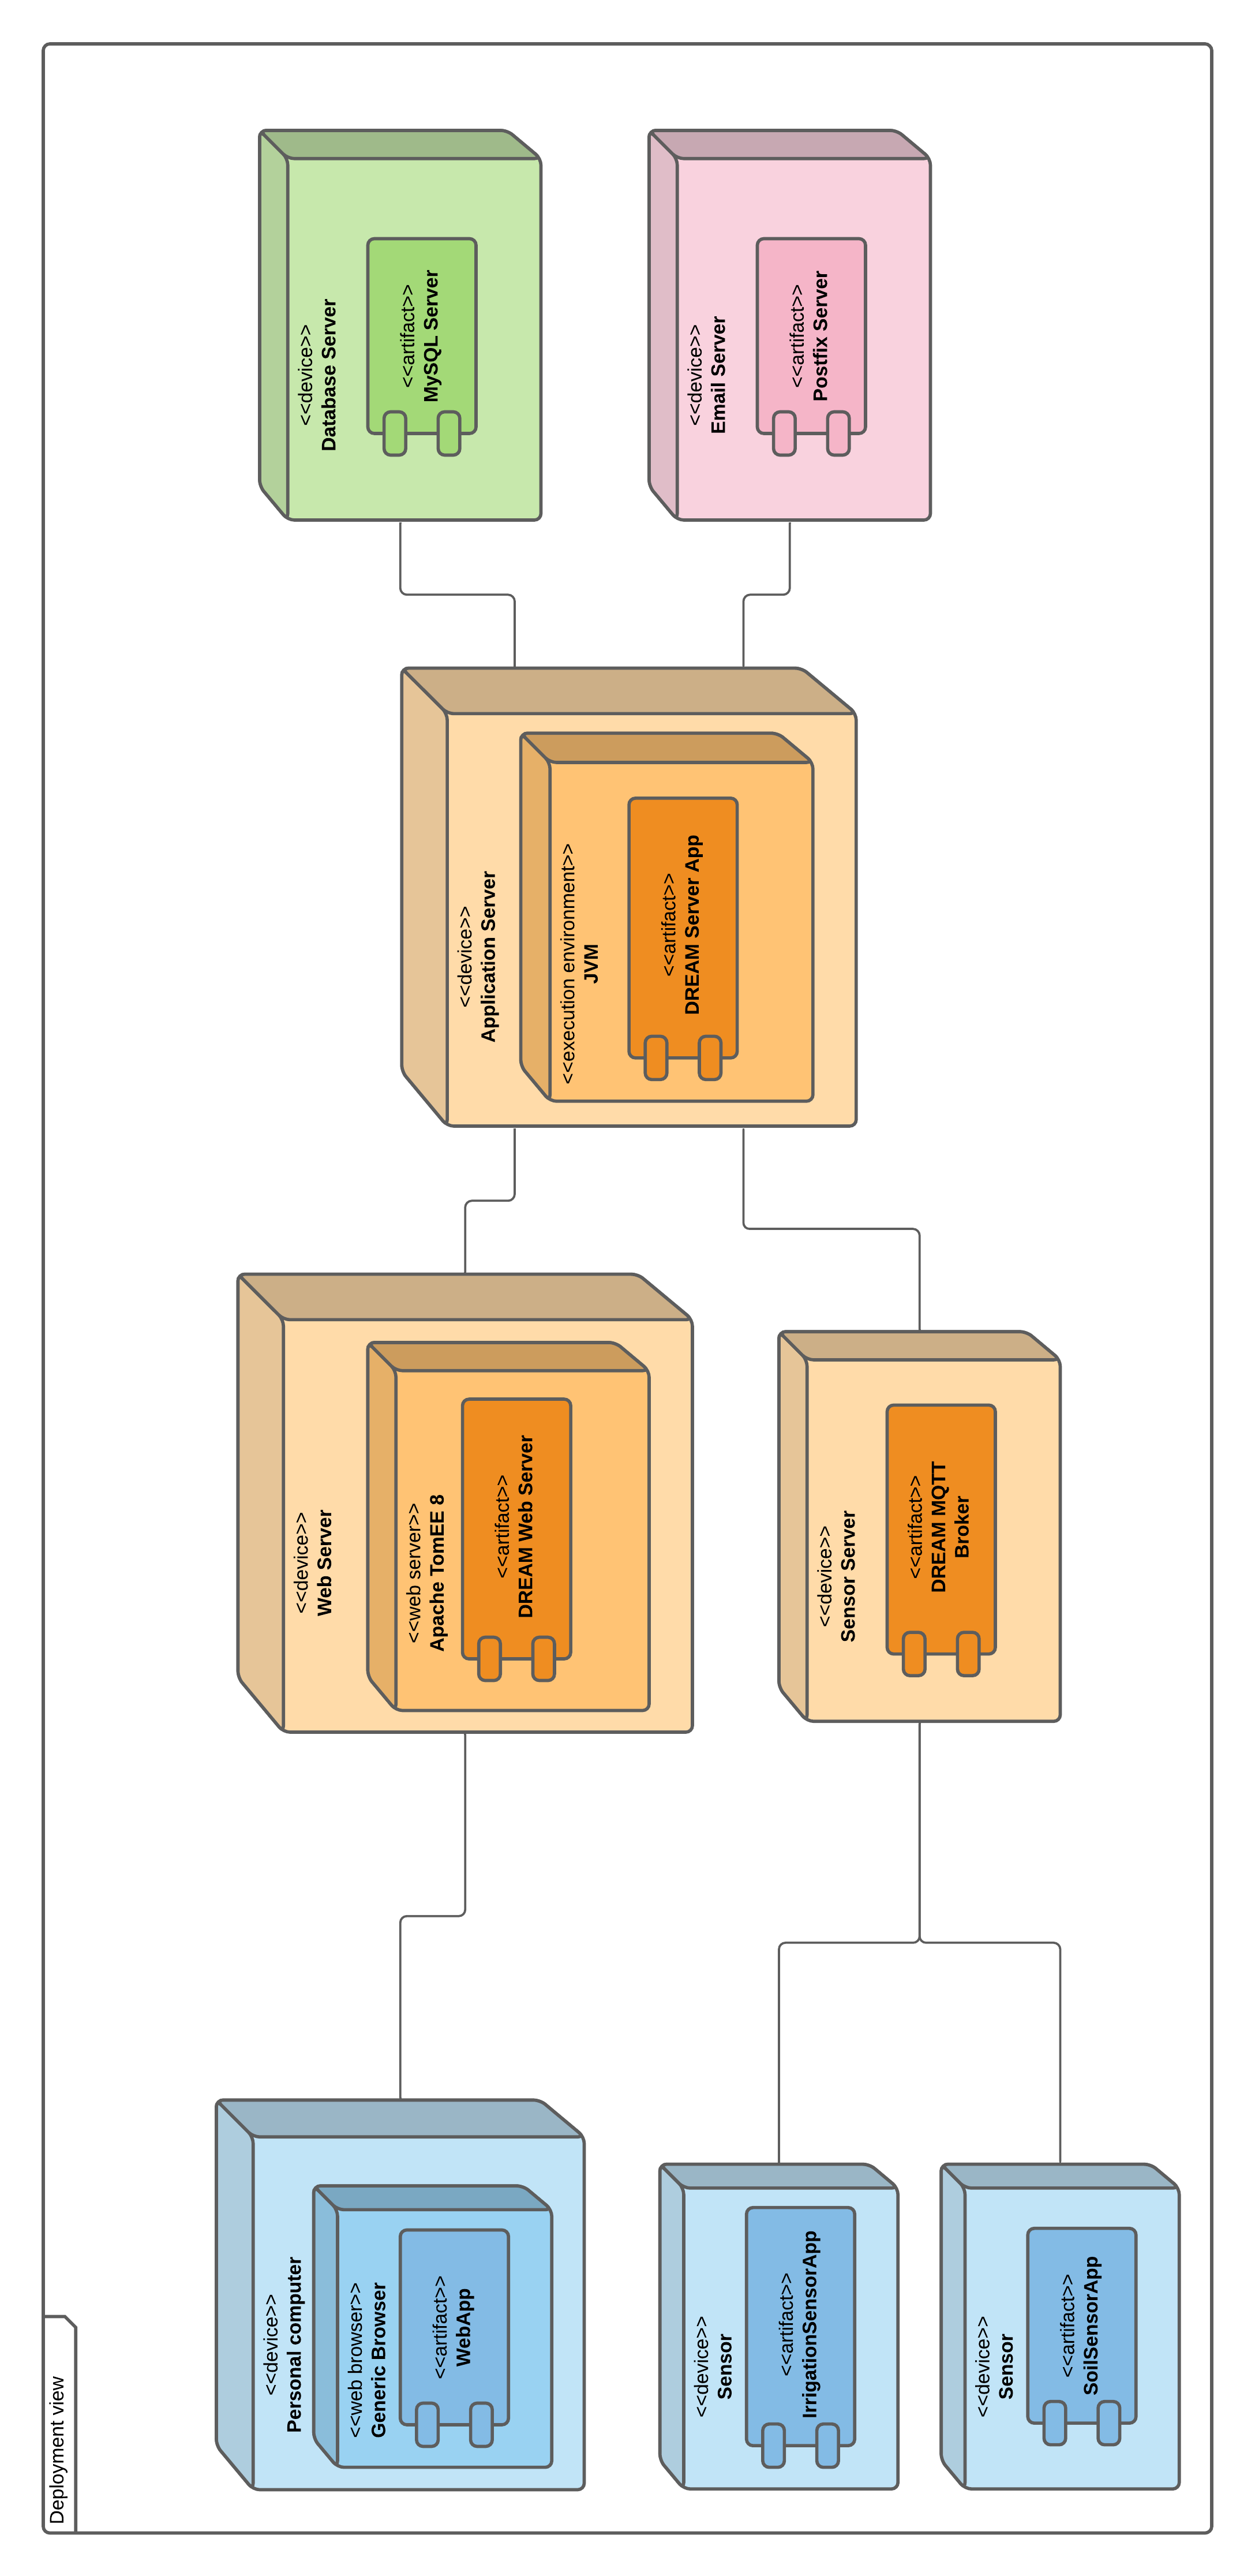
\includegraphics[scale=0.43]{images/deployment.png}
    \caption{Deployment Diagram}
    \label{fig:deployment}
\end{figure}
\subsection{Runtime view}
\subsection{Component Interfaces}
This section lists all the methods exposed by each interface to the external components. Only internal components of the application server are described.
For each method, its parameters and its return value are only meant to give an idea of its behaviour.
\begin{itemize}
    \item \textbf{Farmer Interface}
    \begin{itemize}
        \item handleRequest(httpRequest): HttpResponse
    \end{itemize}
    \item \textbf{PM Interface}
    \begin{itemize}
        \item handleRequest(httpRequest): HttpResponse
    \end{itemize}
    \item \textbf{SH Interface}
    \begin{itemize}
        \item postSensorData(sensorData): void
    \end{itemize}
    \item \textbf{Irrigation Interface}
    \begin{itemize}
        \item postSensorData(sensorData): void
    \end{itemize}
    \item \textbf{Access Manager Interface}
    \begin{itemize}
        \item authUser(email, password): User
        \item getAuthenticatedUser(): User
    \end{itemize}
    \item \textbf{Dashboard Interface}
    \begin{itemize}
        \item getHomepage(): DashboardPage
        \item getReportPage(): DashboardPage
        \item getReportCreationPage(): DashboardPage
        \item getProductListPage(): DashboardPage
        \item getProductPage(): DashboardPage
        \item getForumPage(): DashboardPage
        \item getThreadPage(): DashboardPage
        \item getFarmerPage(): DashboardPage
        \item getHelpRequestListPage(): DashboardPage
        \item getHelpRequestPage(): DashboardPage
        \item getHelpRequestCreationPage(): DashboardPage
        \item getForecastPage(): DashboardPage
        \item getLoginPage(): DashboardPage
        \item setObject(object): void
    \end{itemize}
    \item \textbf{User Manager Interface}
    \begin{itemize}
        \item getUser(userId): User
        \item getUserList(limit): List$<$User$>$ 
    \end{itemize}
    \item \textbf{Forum Interface}
    \begin{itemize}
        \item 
    \end{itemize}
    \item \textbf{HR Interface}
    \begin{itemize}
        \item 
    \end{itemize}
    \item \textbf{Report Interface}
    \begin{itemize}
        \item 
    \end{itemize}
    \item \textbf{Weather Interface}
    \begin{itemize}
        \item 
    \end{itemize}
    \item \textbf{DBM Interface}
    \begin{itemize}
        \item 
    \end{itemize}
\end{itemize}
\subsection{Selected Architectural styles and patterns}
\begin{itemize}
    \item 3 tier client-server
    \item middleware based
    \item rest api  
    \item \textbf{Event based communication for sensors}\\The communication protocol chosen to retrieve 
    data created by IoT sensors is Message Queue Telemetry Transport (MQTT), a standard messaging 
    protocol for the Internet of Things that is extremely lightweight and ideal for connecting remote 
    devices with a small code footprint and minimal network bandwidth. MQTT is a publish/subscribe 
    communication protocol: A topic will be created for each farmer, then the sensors, depending on 
    their geographical location, will publish data to the topics corresponding to the farmers of 
    their interest. In this way it will be possible to access the data created by the sensors divided 
    by each farmer. A MQTT Broker Cluster distributed in the region of Telangana, will take care of 
    the management of sensor data. The application server will be subscribed to all topics and will 
    receive periodically the data, it will then store them in the database to make them always 
    accessible for processing.
    This design provides high scalability because, if we had to resort to replication of the 
    application server, it will be enough to subscribe to all topics the new server to receive 
    all sensor data.
    \begin{figure}[h]
        \centering
        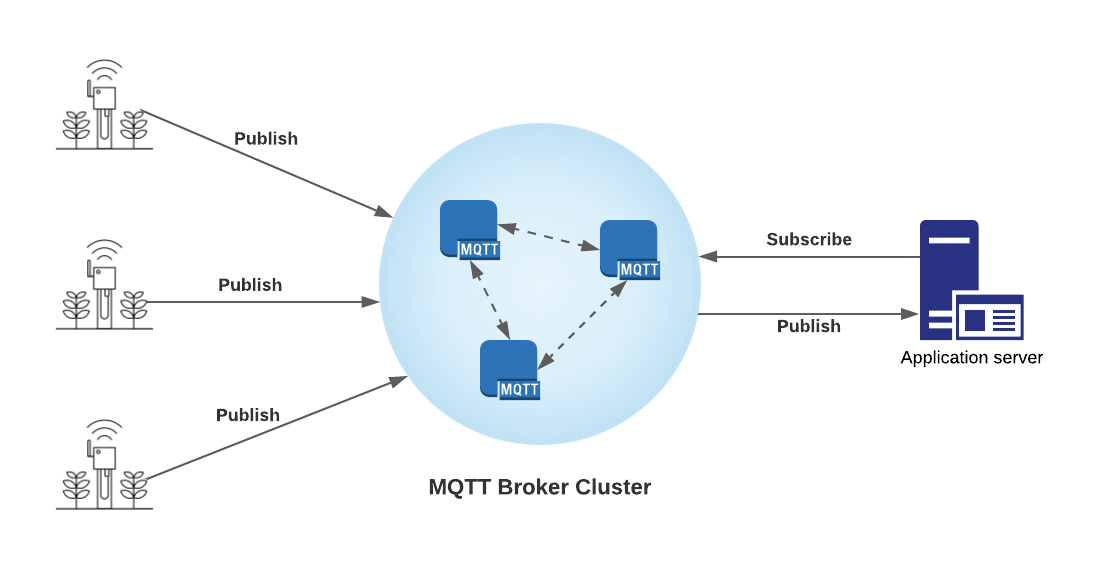
\includegraphics[scale=0.5]{images/mqtt.png}
        \caption{Distributed MQTT Broker System}
        \label{fig:ui_login}
    \end{figure}
\end{itemize}
\subsection{Other design decisions}
\begin{itemize}
    \item thin client
\end{itemize}
\section{User Interface Desgin} %l'impaginazione la facciamo alla fine
The following section describes the user interface of the DREAM webapp. Its goal is to motivate design choices, 
describe each mockup, its content and the flow between the various pages of the application.
The section is divided in three subsections: the first one focuses on the farmer's webapp, the second one on the Policy Maker's webapp
and the third on the flow of the webapp.\\
\begin{figure}[h]
    \centering
    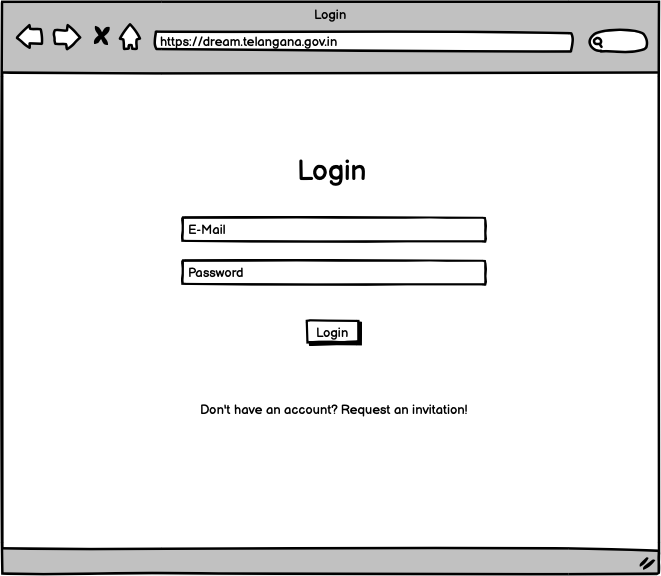
\includegraphics[scale=0.4]{images/uimockups/login.png}
    \caption{Login page}
    \label{fig:ui_login}
\end{figure}
The first page for both farmers and policy makers will always be the login page, requiring e-mail and password to login into the platform.
For farmers, this page will be accessible from any web browser and will also show an option to request an invitation: a simple popup will open up requesting
the user to insert his e-mail address, which will be then submitted to the policy makers who will handle the registration request and procedure.

\subsection{Farmers User Interface}
\begin{figure}[h]
    \centering
    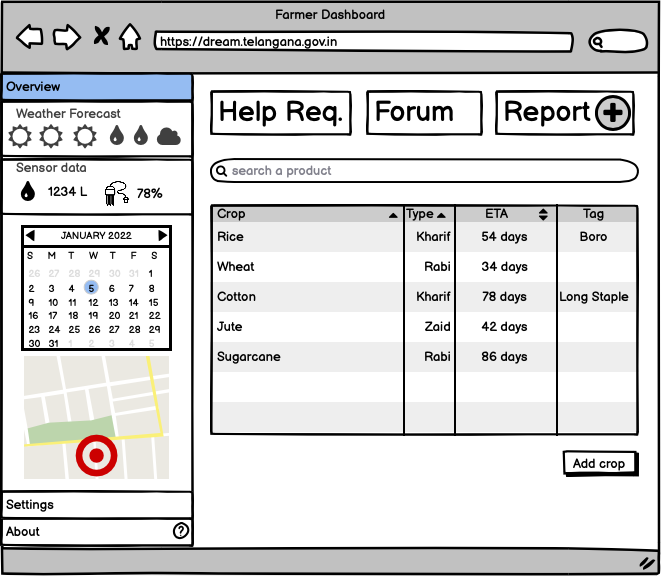
\includegraphics[scale=0.4]{images/uimockups/f_homepage.png}
    \caption{Farmer homepage}
    \label{fig:ui_f_homepage}
\end{figure}
The first page visualized by the farmer once logged in the platform is the homepage. The farmer's homepage contains a brief overview of weather forecasts
and sensor data, and allows users to keep track of their crop in a table containing information about crop's type, eta and comments. The user can add crops 
to the table by clicking "Add crop", which will open a popup to insert the new crop and its info. The page then allows to navigate to the pages for creating reports
and help request, to the forum or to a specific product page by searching the product by its name.\\
\begin{figure}[h]
    \centering
    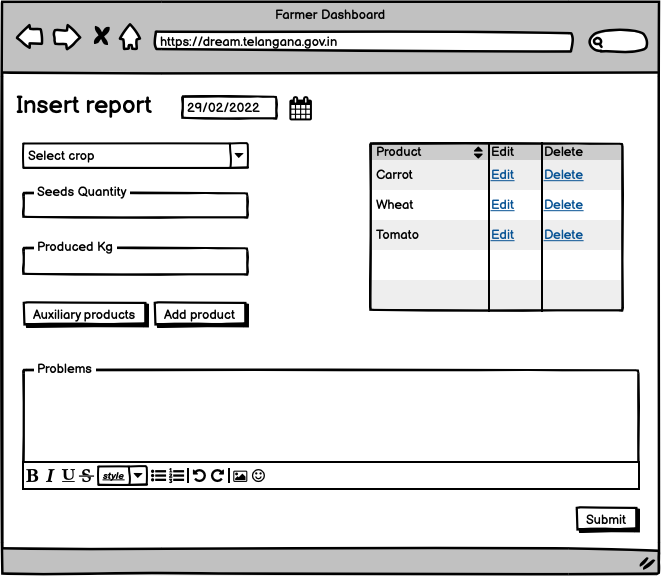
\includegraphics[scale=0.4]{images/uimockups/f_report.png}
    \caption{Farmer's report creation page}
    \label{fig:ui_f_report}
\end{figure}
The report creation page consists of a simple form to insert the harvested products and their quantity. Each product added to the report is visualized 
on a table, that also allows to edit or delete previously added products. To add a product, the user selects the type of product by an interactive dropdown
menu that also allows searching the product, then adds seeds and produced quantity. Clicking on "Auxiliary Products" will open a popup showing the auxiliary
products used in the harvesting process, allowing the user to add, edit or remove them. Once the user has inserted all the necessary information, by clicking on "Add product"
the product will be added to the report's products. The page also contains a text area where the user can insert the problems encountered during the harvesting process. 
Once the report is fully compiled, clicking on "Submit" will create the report and send it to the DREAM server. The webapp will then rediredt the user to the homepage. \\
\begin{figure}[h]
    \centering
    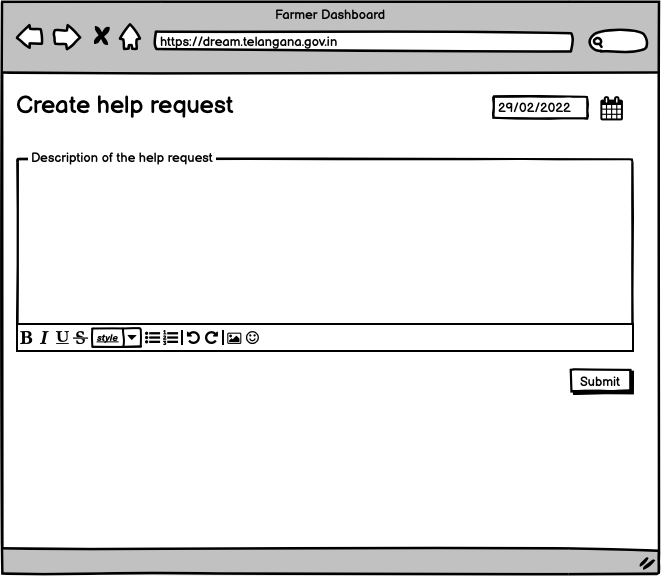
\includegraphics[scale=0.4]{images/uimockups/f_helprequest.png}
    \caption{Farmer's help request creation page}
    \label{fig:ui_f_helprequest}
\end{figure}
\begin{figure}[h]
    \centering
    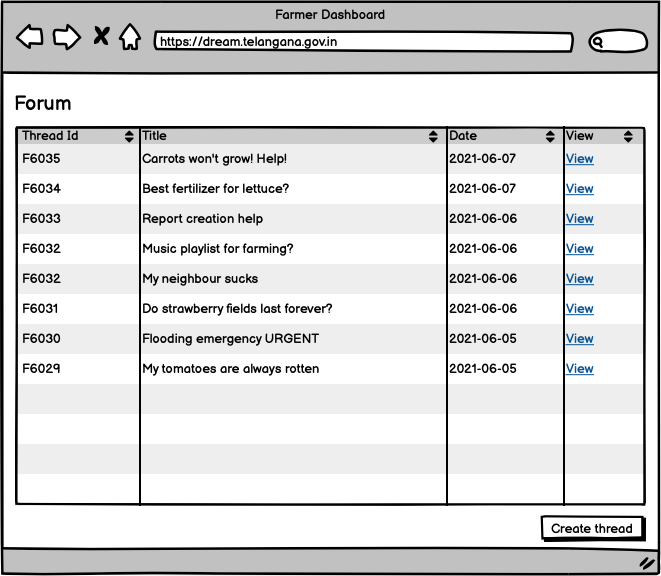
\includegraphics[scale=0.4]{images/uimockups/f_forum.png}
    \caption{Farmer's forum page}
    \label{fig:ui_f_forum}
\end{figure}
The forum page shows all the open threads, allowing the user to open them and visualize the discussion.
A farmer can also create a new thread by clicking "Create thread", which will redirect the user to the thread creation page.\\
\begin{figure}[h]
    \centering
    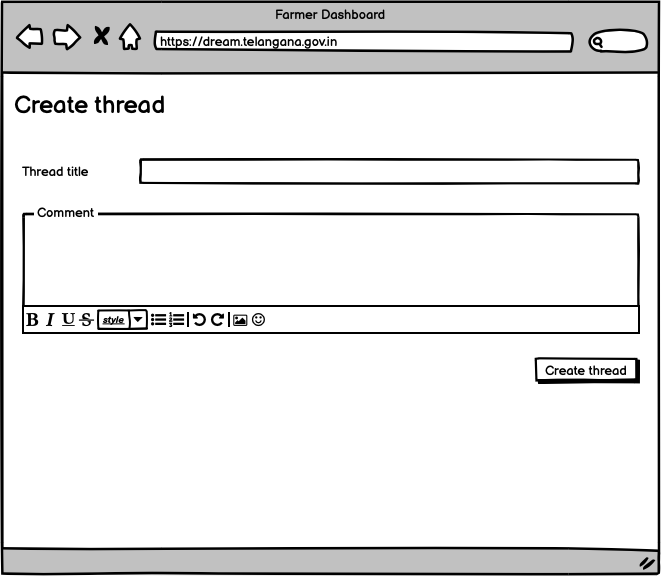
\includegraphics[scale=0.4]{images/uimockups/f_forumcreatethread.png}
    \caption{Farmer's thread creation page}
    \label{fig:ui_f_forumcreatethread}
\end{figure}
\begin{figure}[h]
    \centering
    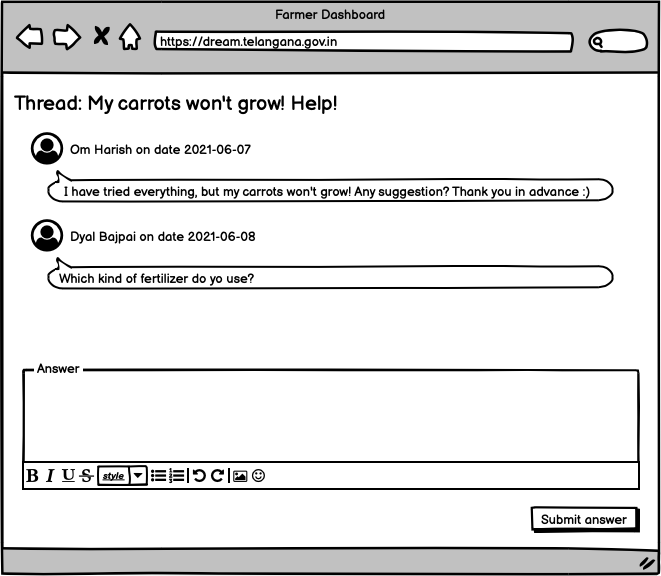
\includegraphics[scale=0.4]{images/uimockups/f_forumthread.png}
    \caption{Farmer's thread page}
    \label{fig:ui_f_forumthread}
\end{figure}
\begin{figure}[h]
    \centering
    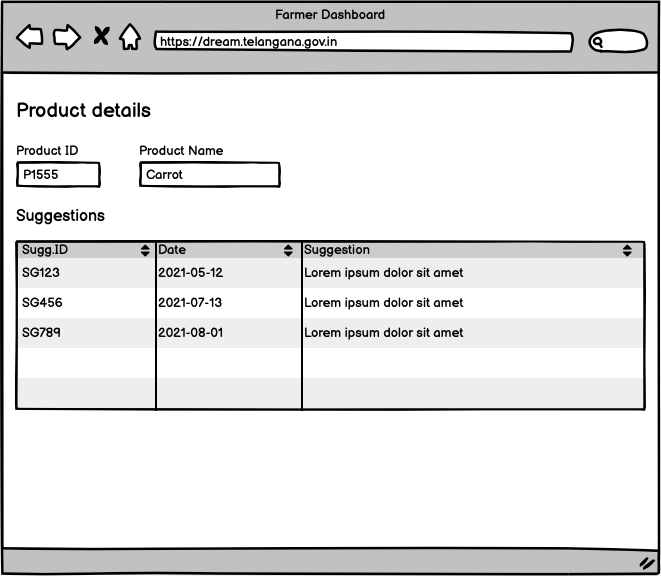
\includegraphics[scale=0.4]{images/uimockups/f_product.png}
    \caption{Farmer's product page}
    \label{fig:ui_f_product}
\end{figure}

\subsection{Policy maker User Interface}
\begin{figure}[h]
    \centering
    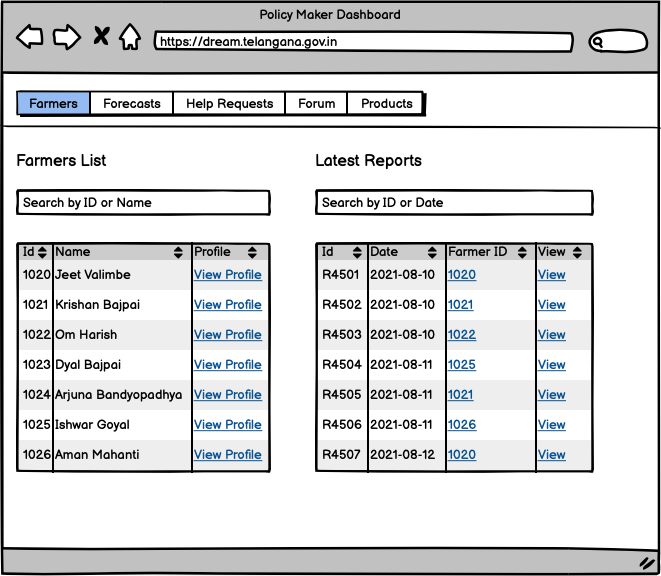
\includegraphics[scale=0.4]{images/uimockups/pm_farmers.png}
    \caption{Policy maker's farmers page}
    \label{fig:ui_pm_farmers}
\end{figure}
The first page visualized by the policy maker once logged into the platform lists the farmers and the latest reports submitted, allowing the
user to search farmers/reports. The user can then navigate to the farmer/report details. On the top of the page there is a navigation bar that
allows the user to switch dashboard page.\\
\begin{figure}[h]
    \centering
    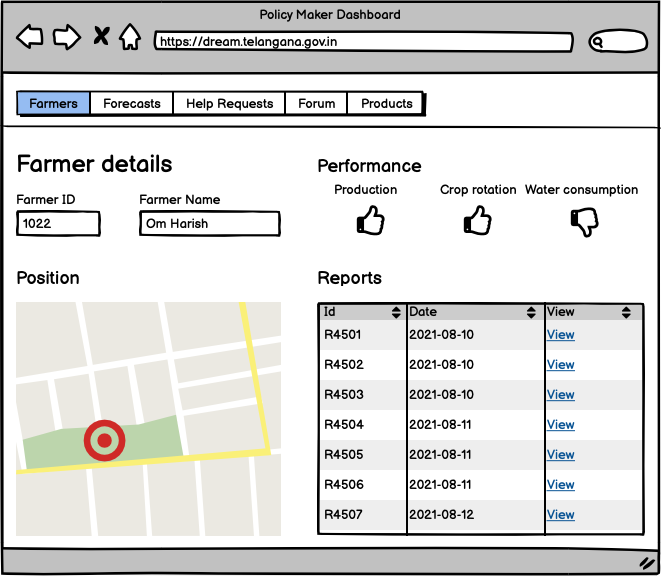
\includegraphics[scale=0.4]{images/uimockups/pm_farmerdetails.png}
    \caption{Policy maker's farmer detail page}
    \label{fig:ui_pm_farmerdetails}
\end{figure}
\begin{figure}[h]
    \centering
    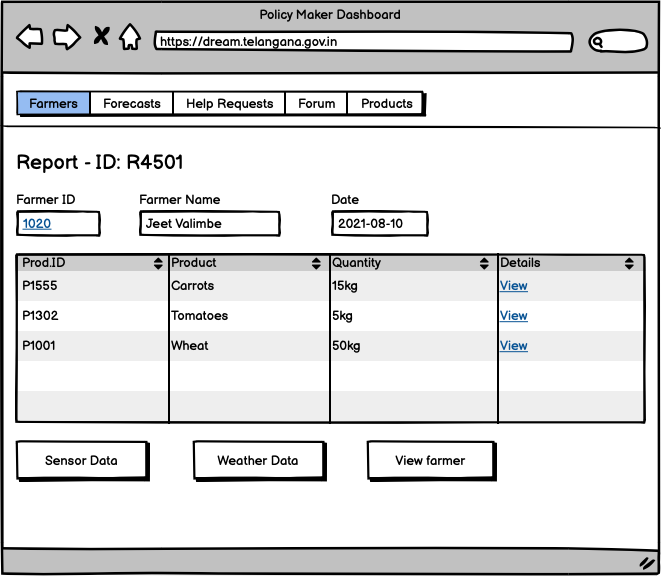
\includegraphics[scale=0.4]{images/uimockups/pm_reports.png}
    \caption{Policy maker's report page}
    \label{fig:ui_pm_reports}
\end{figure}
\begin{figure}[h]
    \centering
    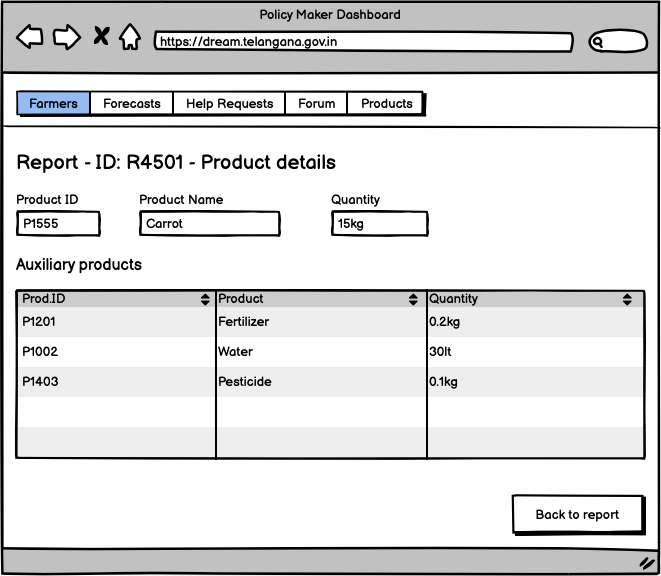
\includegraphics[scale=0.4]{images/uimockups/pm_reportproductdetail.png}
    \caption{Policy maker's report production detail page}
    \label{fig:ui_pm_reportproductdetail}
\end{figure}
\begin{figure}[h]
    \centering
    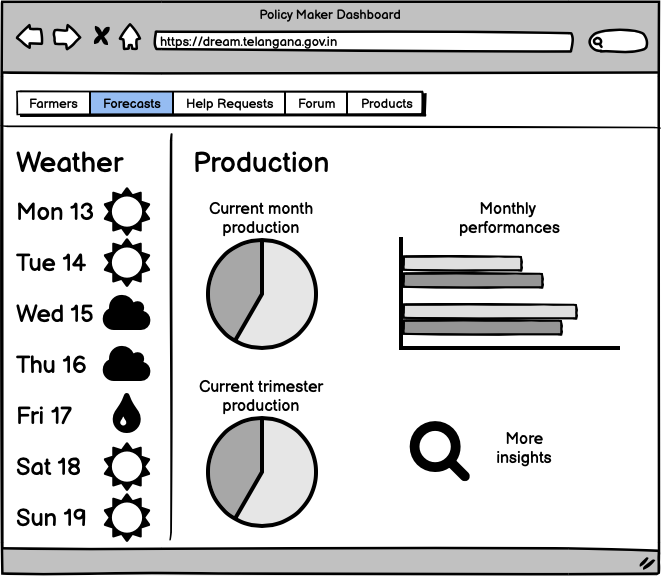
\includegraphics[scale=0.4]{images/uimockups/pm_forecasts.png}
    \caption{Policy maker's forecasts page}
    \label{fig:ui_pm_forecasts}
\end{figure}
The forecast page contains basic information about the future weather forecasts. Production forecasts are calculated and then shown to the user through
graphs.\\
\begin{figure}[h]
    \centering
    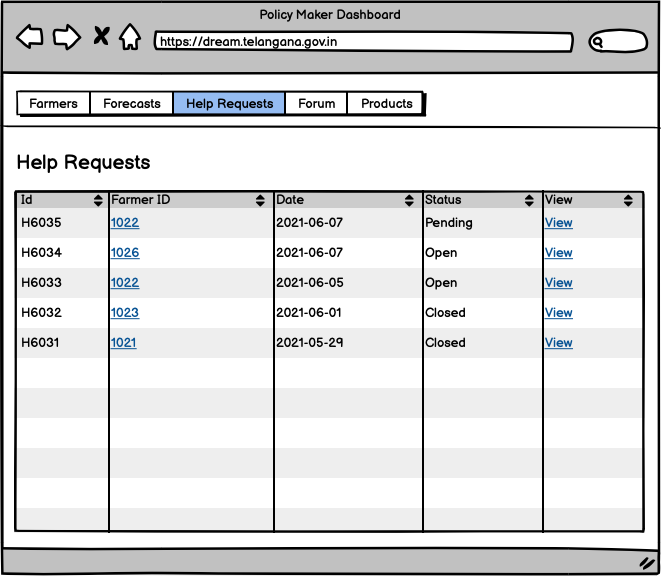
\includegraphics[scale=0.4]{images/uimockups/pm_helprequests.png}
    \caption{Policy maker's help requests page}
    \label{fig:ui_pm_helprequests}
\end{figure}
\begin{figure}[h]
    \centering
    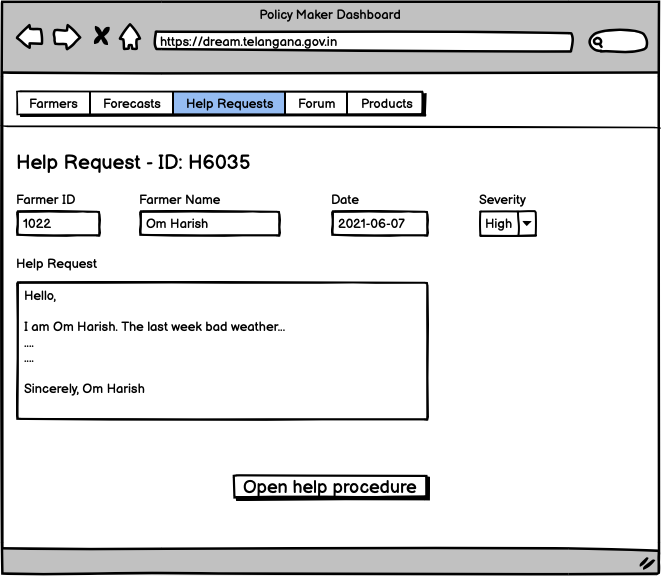
\includegraphics[scale=0.4]{images/uimockups/pm_helprequestdetail.png}
    \caption{Policy maker's help request detail page}
    \label{fig:ui_pm_helprequestdetail}
\end{figure}
\begin{figure}[h]
    \centering
    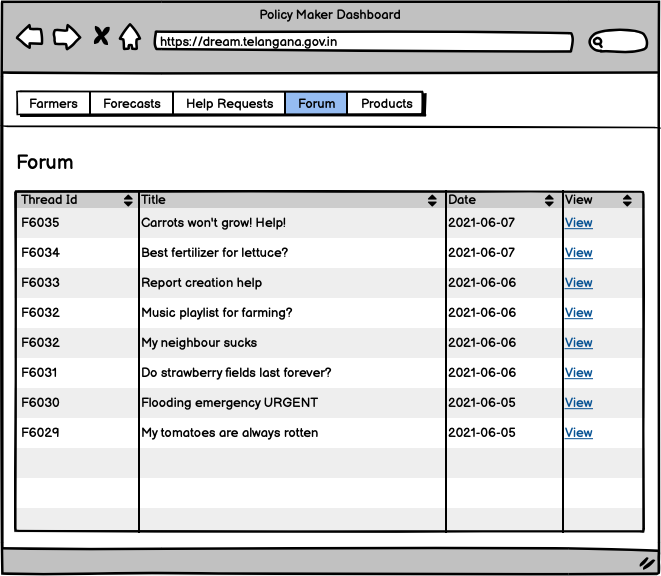
\includegraphics[scale=0.4]{images/uimockups/pm_forum.png}
    \caption{Policy maker's forum page}
    \label{fig:ui_pm_forum}
\end{figure}
\begin{figure}[h]
    \centering
    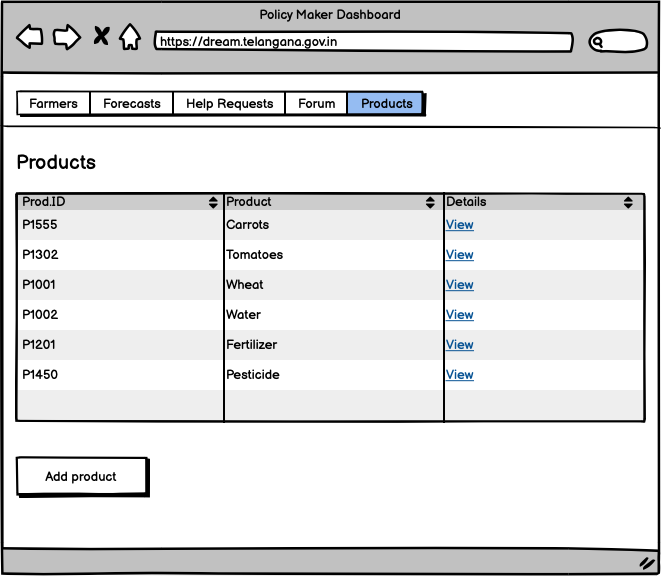
\includegraphics[scale=0.4]{images/uimockups/pm_products.png}
    \caption{Policy maker's products page}
    \label{fig:ui_pm_products}
\end{figure}
\begin{figure}[h]
    \centering
    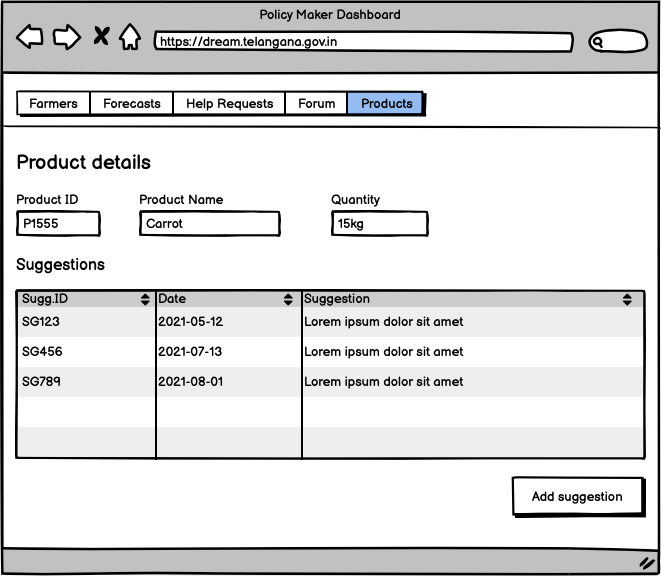
\includegraphics[scale=0.4]{images/uimockups/pm_productdetail.png}
    \caption{Policy maker's product detail page}
    \label{fig:ui_pm_productdetail}
\end{figure}

\subsection{Flow of the User Interface}
\begin{figure}[h]
    \centering
    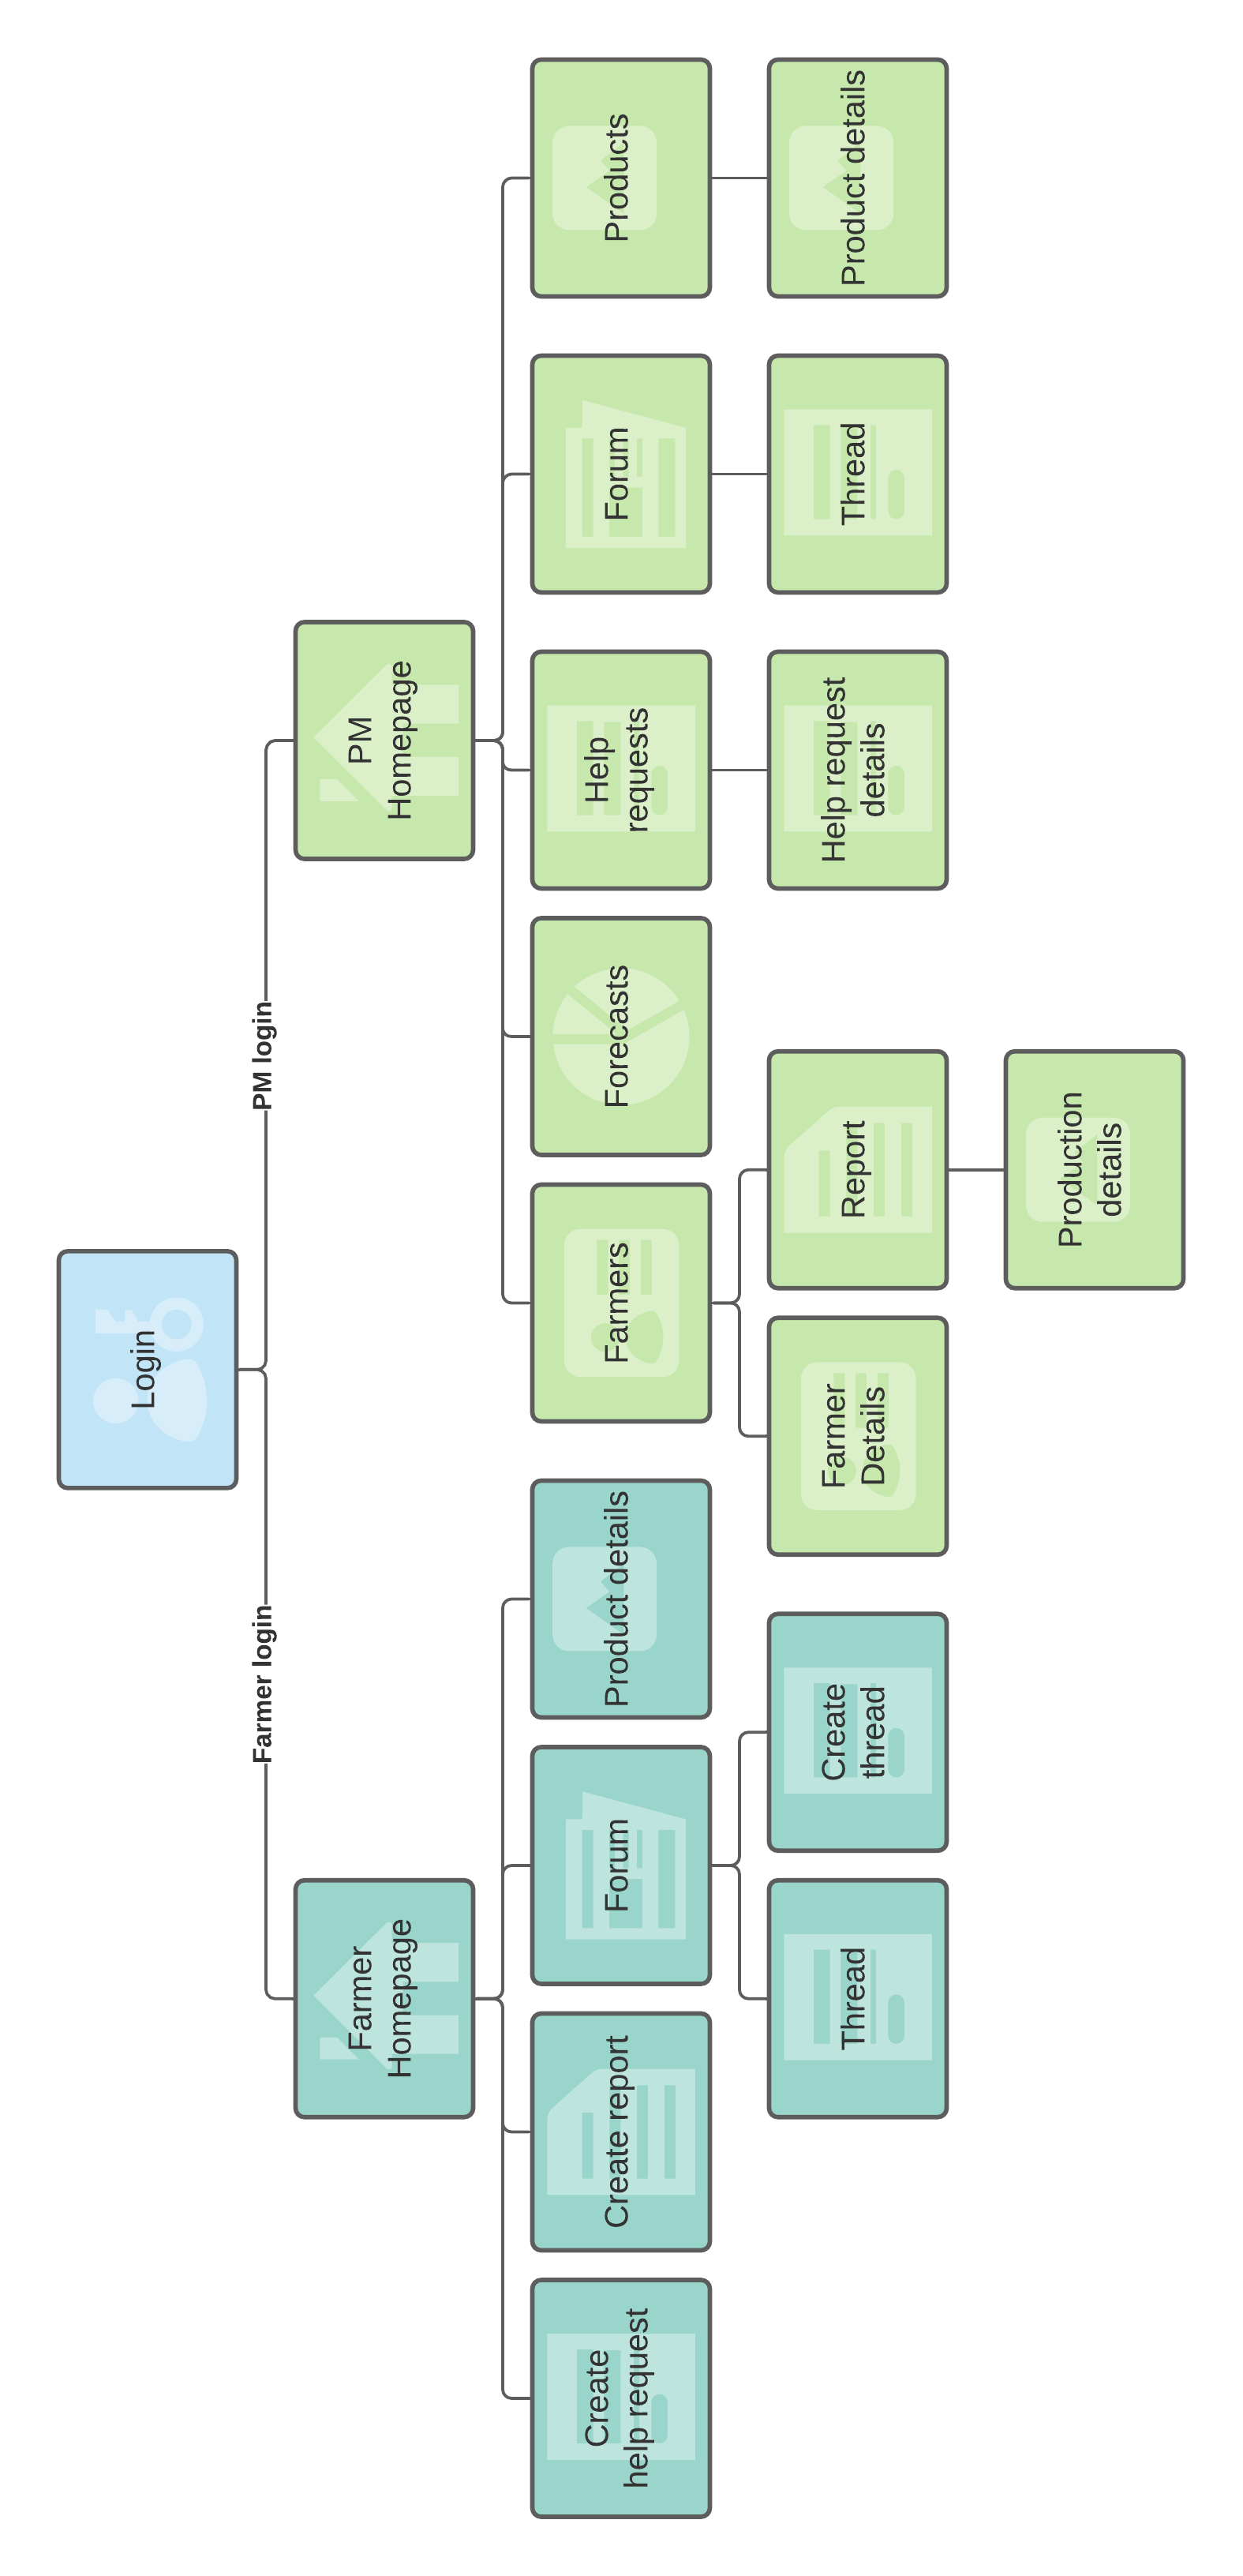
\includegraphics[scale=0.6]{images/uimockups/ui_flow.png}
    \caption{User interface flow}
    \label{fig:ui_flow}
\end{figure}
\section{Requirements Traceability}

\section{Implementation, integration and test plan}

\section{Effort spent}

\bibliography{main.bib}

\end{document}